\documentclass[a4paper,10pt]{article}

\usepackage{fancyheadings}
%figure insertion
\usepackage{graphicx}
\usepackage{tikz}
\usepackage{pgfplots}

%%%%%%%%%%%%%%%%%%%%%%%%%%%%%%%%%%%%%%%%%%%%%%%%%%%%%%%%%%%%%%%%%%%
%
\setlength\textheight{9in}
\setlength\textwidth{6.5in}
\setlength\headwidth{6.5in}
\setlength\oddsidemargin{0in}
\setlength\evensidemargin{0in}
\setlength\marginparwidth{0in}
\setlength\topmargin{0in}
%
\begin{document}
%
%%%%%%%%%%%%%%%%%%%%%%%%%%%%%%%%%%%%%%%%%%%%%%%%%%%%%%%%%%%%%%%%%%%
\begin{figure}[!t]
  \centering
	\pgfplotsset{every axis/.append style={font=\footnotesize, thin, tick style={ultra thin}}}
	 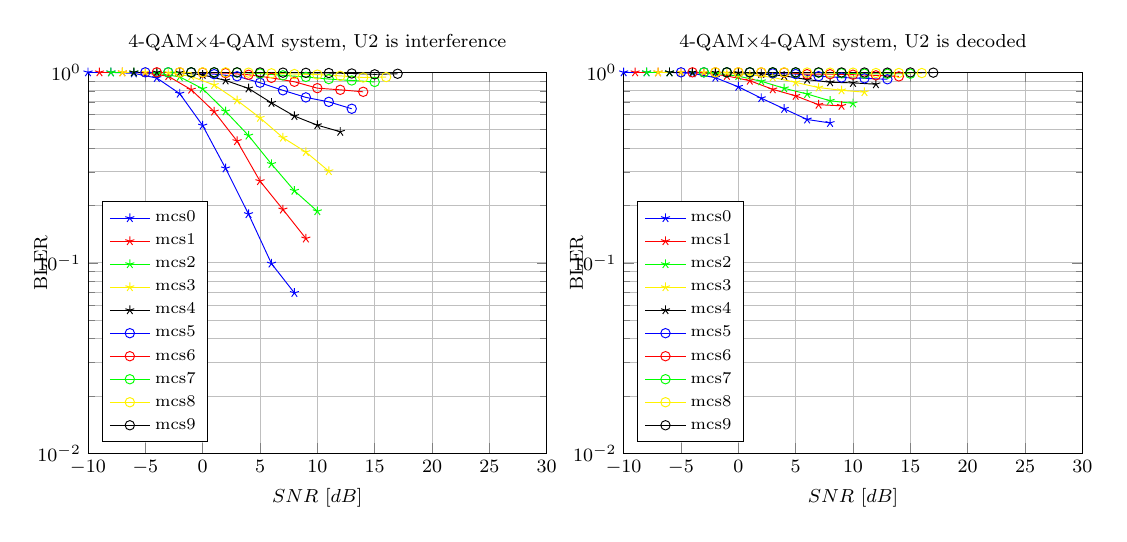
\begin{tikzpicture}[scale=0.85][font=\footnotesize]
		\pgfplotsset{	every axis y label/.append style={yshift=-10pt}}
		\pgfplotsset{	every axis legend/.append style={cells={anchor=west},font=\scriptsize}}
		\tikzstyle{every axis legend}+=[cells={anchor=west}]
		\tikzstyle{every axis legend}+=[at={(0.03,0.03)},anchor=south west,font=\scriptsize]
		\begin{semilogyaxis}[
			title={4-QAM$\times$4-QAM system, U2 is interference},
			xlabel={$SNR~[dB]$},
			ylabel={BLER},
			grid={both},
			ymin={1e-2},
			ymax={1e0},
			% ytick={0.0090527, -0.0059613,...,0.000001061,
			xmin={-10},
			xmax={30},
			xtick={-10, -5,...,30},
			name=plot1,]

%User2=0,Channel=C,MCS=[0 1 2 3 4 5 6 7 8 9],NFRAMES=5000
\addplot[color=blue, mark=star] plot coordinates {(-10.000000,1.000000)(-8.000000,0.999600)(-6.000000,0.987210)(-4.000000,0.933653)(-2.000000,0.772982)(0.000000,0.525580)(2.000000,0.313349)(4.000000,0.180256)(6.000000,0.099121)(8.000000,0.069544)};
\addplot[color=red, mark=star] plot coordinates {(-9.000000,1.000000)(-7.000000,1.000000)(-5.000000,0.992806)(-3.000000,0.953637)(-1.000000,0.810951)(1.000000,0.622702)(3.000000,0.435651)(5.000000,0.268585)(7.000000,0.190647)(9.000000,0.134293)};
\addplot[color=green, mark=star] plot coordinates {(-8.000000,1.000000)(-6.000000,0.999600)(-4.000000,0.989209)(-2.000000,0.946443)(0.000000,0.820144)(2.000000,0.623901)(4.000000,0.465627)(6.000000,0.330136)(8.000000,0.239009)(10.000000,0.186651)};
\addplot[color=yellow, mark=star] plot coordinates {(-7.000000,1.000000)(-5.000000,1.000000)(-3.000000,0.995604)(-1.000000,0.951239)(1.000000,0.858513)(3.000000,0.712230)(5.000000,0.577138)(7.000000,0.454037)(9.000000,0.381695)(11.000000,0.302958)};
\addplot[color=black, mark=star] plot coordinates {(-6.000000,1.000000)(-4.000000,1.000000)(-2.000000,0.997202)(0.000000,0.970024)(2.000000,0.906475)(4.000000,0.822942)(6.000000,0.691447)(8.000000,0.589528)(10.000000,0.527978)(12.000000,0.487610)};
\addplot[color=blue, mark=o] plot coordinates {(-5.000000,1.000000)(-3.000000,1.000000)(-1.000000,0.998801)(1.000000,0.978018)(3.000000,0.953637)(5.000000,0.881695)(7.000000,0.804556)(9.000000,0.738609)(11.000000,0.699840)(13.000000,0.643885)};
\addplot[color=red, mark=o] plot coordinates {(-4.000000,1.000000)(-2.000000,1.000000)(0.000000,0.996803)(2.000000,0.990408)(4.000000,0.970823)(6.000000,0.935252)(8.000000,0.892086)(10.000000,0.825739)(12.000000,0.809353)(14.000000,0.790168)};
\addplot[color=green, mark=o] plot coordinates {(-3.000000,1.000000)(-1.000000,1.000000)(1.000000,0.999600)(3.000000,0.997602)(5.000000,0.985612)(7.000000,0.964029)(9.000000,0.945643)(11.000000,0.921663)(13.000000,0.906075)(15.000000,0.890088)};
\addplot[color=yellow, mark=o] plot coordinates {(-2.000000,1.000000)(0.000000,1.000000)(2.000000,1.000000)(4.000000,0.996003)(6.000000,0.988010)(8.000000,0.979217)(10.000000,0.972822)(12.000000,0.958034)(14.000000,0.939249)(16.000000,0.944444)};
\addplot[color=black, mark=o] plot coordinates {(-1.000000,1.000000)(1.000000,1.000000)(3.000000,0.999600)(5.000000,0.998801)(7.000000,0.996003)(9.000000,0.994005)(11.000000,0.991607)(13.000000,0.986011)(15.000000,0.976019)(17.000000,0.982814)};

			\legend{{mcs0},{mcs1},{mcs2},{mcs3},{mcs4},{mcs5},{mcs6},{mcs7},{mcs8},{mcs9}}
		\end{semilogyaxis}
%
		\begin{semilogyaxis}[
			title={4-QAM$\times$4-QAM system, U2 is decoded},
			xlabel={$SNR~[dB]$},
			ylabel={BLER},
			grid={both},
			ymin={1e-2},
			ymax={1e0},
			% ytick={0.0090527, -0.0059613,...,0.000001061,
			xmin={-10},
			xmax={30},
			xtick={-10, -5,...,30},
			at=(plot1.right of south east), anchor=left of south west,]

%User2=1,Channel=C,MCS=[0 1 2 3 4 5 6 7 8 9],NFRAMES=5000
\addplot[color=blue, mark=star] plot coordinates {(-10.000000,1.000000)(-8.000000,1.000000)(-6.000000,0.999201)(-4.000000,0.987610)(-2.000000,0.937250)(0.000000,0.839329)(2.000000,0.731815)(4.000000,0.643086)(6.000000,0.565548)(8.000000,0.542366)};
\addplot[color=red, mark=star] plot coordinates {(-9.000000,1.000000)(-7.000000,1.000000)(-5.000000,1.000000)(-3.000000,0.992006)(-1.000000,0.957634)(1.000000,0.903677)(3.000000,0.814149)(5.000000,0.752198)(7.000000,0.676259)(9.000000,0.667066)};
\addplot[color=green, mark=star] plot coordinates {(-8.000000,1.000000)(-6.000000,1.000000)(-4.000000,0.998401)(-2.000000,0.988409)(0.000000,0.954836)(2.000000,0.897282)(4.000000,0.824540)(6.000000,0.769384)(8.000000,0.709033)(10.000000,0.687050)};
\addplot[color=yellow, mark=star] plot coordinates {(-7.000000,1.000000)(-5.000000,1.000000)(-3.000000,0.999201)(-1.000000,0.994404)(1.000000,0.970024)(3.000000,0.940847)(5.000000,0.885292)(7.000000,0.831735)(9.000000,0.804556)(11.000000,0.786970)};
\addplot[color=black, mark=star] plot coordinates {(-6.000000,1.000000)(-4.000000,1.000000)(-2.000000,0.999201)(0.000000,0.994804)(2.000000,0.981215)(4.000000,0.958433)(6.000000,0.915667)(8.000000,0.887290)(10.000000,0.880096)(12.000000,0.866107)};
\addplot[color=blue, mark=o] plot coordinates {(-5.000000,1.000000)(-3.000000,1.000000)(-1.000000,0.999600)(1.000000,0.998401)(3.000000,0.987210)(5.000000,0.979217)(7.000000,0.954037)(9.000000,0.938849)(11.000000,0.930056)(13.000000,0.919265)};
\addplot[color=red, mark=o] plot coordinates {(-4.000000,1.000000)(-2.000000,1.000000)(0.000000,0.999600)(2.000000,0.998801)(4.000000,0.996803)(6.000000,0.978018)(8.000000,0.977218)(10.000000,0.971623)(12.000000,0.964029)(14.000000,0.952038)};
\addplot[color=green, mark=o] plot coordinates {(-3.000000,1.000000)(-1.000000,1.000000)(1.000000,1.000000)(3.000000,0.999600)(5.000000,0.997202)(7.000000,0.995204)(9.000000,0.989209)(11.000000,0.983613)(13.000000,0.982414)(15.000000,0.982814)};
\addplot[color=yellow, mark=o] plot coordinates {(-2.000000,1.000000)(0.000000,1.000000)(2.000000,1.000000)(4.000000,1.000000)(6.000000,0.997602)(8.000000,0.996003)(10.000000,0.996003)(12.000000,0.991607)(14.000000,0.992006)(16.000000,0.991207)};
\addplot[color=black, mark=o] plot coordinates {(-1.000000,1.000000)(1.000000,1.000000)(3.000000,1.000000)(5.000000,1.000000)(7.000000,0.999201)(9.000000,0.998401)(11.000000,0.997602)(13.000000,0.996003)(15.000000,0.998401)(17.000000,0.996003)};

			\legend{{mcs0},{mcs1},{mcs2},{mcs3},{mcs4},{mcs5},{mcs6},{mcs7},{mcs8},{mcs9}}
		\end{semilogyaxis}
	\end{tikzpicture}
 	\caption{BLER as a function of SNR, LCM Max-Log MAP detectors, SCM-C channel.}
  \label{fig:testScmC}
\end{figure}
%
%%%%%%%%%%%%%%%%%%%%%%%%%%%%%%%%%%%%%%%%%%%%%%%%%%%%%%%%%%%%%%%%%%%
\end{document}
